\chapter{Belle II Upgrade}

This second chapter wants to adress some of the main reasons in favor of the upgrade of Belle II. We will give an overview of the primary background sources in the experiment to understand how to mitigate them to be able to achieve a better performance of the whole detector, even ramping up the luminosity. Eventually we will also introduce some of the proposes made for the vertex detector, which is the focus of this thesis.


%---------------------------------------------
%			2.1
%---------------------------------------------
\section{Background sources and limitations in Belle II}

SuperKEKB is already the world's highest-luminosity collider and it aims to reach a new luminosity peak and to increase the statistics in the future, to become more sensitive to rare process and precise measurements of Belle II physics program. 
But to be able to do this without loosing the good functionality of the entire detector, it's necessary to understand how to mitigate the beam backgrounds where possible and how to cope with the consequent challenges.

Several simulations and measurements of beam background are still being done in order to guess possible future machine scenarios, under new luminosity conditions.
This is necessary to study the vulnerability of the subdetectors (and more generally of the machine) and so to design the countermeasures to adopt against the deterioration of performance and material.


\subsection{Major background sources}

Making clear that even the interaction of the beams is a source of noise for the measurements, in the following are listed some of the \textit{beam-induced} and \textit{luminosity-dependent} background sources.


\begin{description}
\item[Touschek effect]: 
	It is an intra-bunches scattering process, where the Coulomb scattering of two particles in the same beam bunch causes a variation of their energies, increasing the value of one of them and lowering that of the other from the nominal value. This interaction among the bunch particles is the first beam background source at SuperKEKB.
\item[Beam-gas scattering]: 
	this represents the collision of beam particles with residual gas molecules in the beam pipe. It's the second beam background source and it can occur via two processes: Coulomb interactions, which changes the direction of the beam particles, and bremsstrahlung scattering, which instead decreases their energy. 
\end{description}
	
Because of these two processes, the scattered particle fall out the stable orbit and hit the beam pipe while they move around the ring. This causes electromagnetic showers that could reach the detector if their origin (loss position) is close to it.


\begin{description}
\item[Radiative Bhabha scattering and two-photon processes]:
	There are several undesirable collision processes at IP, which have very high cross sections but only little interest for the physics studied in the experiment. Two of them are \textbf{Bhabha scattering} ($e^{+}e^{-} \rightarrow e^{+}e^{-} \lambda$) and \textbf{Two-photon processes} ($e^{+}e^{-} \rightarrow e^{+}e^{-}e^{+}e^{-} $). 
	In the first effect the emitted photon interacts with the iron magnets and produces a very large amounts of neutrons via the photo-nuclear resonance mechanism. [Such neutrons are the main background source for the outermost Belle II detector, the $K_{L}$ and muon detector (KLM).] The electrons-positrons pairs of the latter instead, can spiral around the solenoid field lines and leave multiple hits in the inner Belle II detectors.\\
	
These processes increase the Belle II occupancy and radiation dose, and they are reffered as \textit{Luminosity background} because their strenght is proportional to the luminosity. The future upgrade intends to deal with this problem in order to keep occupancy low.

\item[Synchrotron Radiation (SR)]:
	X-rays emitted from the beam when electrons and positrons pass through the strong magnetic field near the IP. The HER beam is the main source of this type of background, because SR power is proportional to the square of beam energy and magnetic field.
SR can potentially damage the inner layers of the vertex detector due to an higher radiation dose. As a matter of fact, many current studies aim to enhance radiation hardness detector.
\end{description}

There are also other  background sources beyond those mentioned aboce and during the last decade a well-structured set of countermeasures have been developed trying to ease each one of them.


\subsection{Current background status and future implications (predictions)}

Several monitoring devices are located all along the accelerator to keep under control radiation doses on both detector and delicate regions of the ring, to intervene as soon as possible in case too high levels are reached. Indeed large doses of radiation could cause accidental damages on the detector, decreasing its performance.

Event though the current level is of no concern in terms of occupancy for the innermost layers of the vertex detector, in the case of a larger amount, such as of SR may cause inhomogenities in PXD module, which would make more difficult to compensate them by adjusting the operation voltages of the affected ones.

Until now it can be said that SuperKEKB and Belle II are operating stably. Beam-induced backgorund rates are well below the limits of the detector and do not prevent from increasing further tha current and hence the luminosity.  
Despite that, there are several other difficulties that can limit beam currents and so the possibility to move the luminosity frontier at towards higher levels, allowing Belle II reaserchers to study rare physics processes. 


%SEU??

%---------------------------------------------
%			2.2
%---------------------------------------------
\section{Purposes of the upgrade}

Current studies foresee that SuperKEKB may reach higher luminosity targets with the existing accelerator complex (background simulations have been done for each phase listed in section \vpageref{perspectives}), but in order to achieve the estabilished final value of  \num{6.3e-35} $cm^{-2} s^{-1}$ by 2030, an enhancement of the interaction region are under consideration.\\

Belle II detector is also designed to operate efficiently under the high levels of backgrounds extrapolated to luminosity target, but safety margins are not so large. Moreover in the case of a redesign of the interaction region large uncertainties in the background extrapolations are unavoidable. \\
Therefore the global upgrade program is justified by many considerations, among them:

\begin{itemize}
\item improve detector's resitance to higher level of background;
\item make each subdetectors long-lived against radiation damage;
\item push forward safety margins for running at higher luminosity;
\item develop the technology to cope with different future paths;
\item improve overall physics performance.
\end{itemize}


In particular all different upgrade ideas of the whole Belle II detector intend to ensure its proper functioning, at the higher level of luminosity ever achived, condering also further improvements of the lattice machine and so of the colliding beams. Indeed current detector configuration is not expected to maintain its performance level when facing high beam background level or high rates.

In regards to the Vertex Detector, all proposed improvements aim to:

\begin{itemize}
\item reduce occupancy level by employing fully pixelated and fast detector (nowadays CMOS technologies are the most probably choice);
\item increase robustness against tracking efficiency and resolution losses from beam background;
\item improve radiation hardness for delaying detector ageing effects and so performance degradation;
\item reduce the inserted material budget between subdetectors in order to achieve good resolution lessening the multiple scattering, above all at lower momenta.
\end{itemize}




%---------------------------------------------
%			2.3
%---------------------------------------------
\section{Summary of possible VXD upgrade}

%PHYSICS PERFORMANCE????
\begin{comment}
In particular there are three fundamental aspects in physics performance (concern) in regards to VXD and its upgrade:

\begin{itemize}
\itemsep0em
\item Low momentum track finding; 
\item Vertex and IP resolution;
\item Triggers.
\item integration time
\end{itemize}

\end{comment}

The Vertex Detector is particularly sensitive to machine background, beeing the closest to the beam pipe and therefore subject to high doses of radiation.
As we have already seen, current studies are trying to extrapolate how it could be affected by reaching the future luminosity target, but there are a lot of uncertainties due to models and still not well defined design of the interaction region. Moreover a completely new detector might be required, in event of a considerable(significant) redesing of the IR. However in this case, also the physics performance could be improved, taking advantage of the more recent technology developments.\\

In the following we will present in a few words the four main proposal for future upgrade: DEPFET pixel, thin sensor, CMOS MAPS pixel and SOI technology.

%ALCUNI GIA' ABBANDONATI?


\subsection{DEPFET}

This first proposal intend to minimize risk and costs of the project, preserving the general layout of the PXD system. The upgrade consists to improve the sensor above all, in order to provide higher safety factor for the allowed occupancy and to prevent some issue that at the moment weaken the good functionality of the detector.

Some of the main improvements are listed below:

\begin{itemize}
\item improve signal trasmission on the pixel matrix and the signal processing in the read-out, in order to reduce the read-out time per row from the current 100 ns to 50 ns. In this way the frame time and the background occupancy might be reduce by factor 2, while leaving unchanged the optimized pixel size and number of PXD as it stands;
\item increase the robustness against beam losses which could make inefficient or even inoperative gate lines on almost all PXD modules. This reaction seems to be due to a high photocurrent on the chip because of the high istantaneous dose. it could be mitigate by adding protection circuits on-chip;
\item TID effect on the chip provokes an unexpected avalanche current that does not compromise the sensor performance but requires more power supply to provide ennough current. This issue might be solved by bringing some changes in the DEPFET pixel layout.
\end{itemize}

Simulations and studies of the new pixel design are showing promising results.???


\subsection{Thin and Fine-Pitch SVD}

The Thin and Fine-Pitch SVD (\textbf{TFP-SVD}) is a new detector concept that aims to improve not only SVD, but also the inner part of the CDC, whose functionality could be threatened by future beam background condition.
This proposal takes into accout the Double-sided Silicon Strip Detector (DSSD) as a prime candidate for a tracking device in the inner and middle detector volume since a single sensor can cover a large dimension of about 100x100 $mm^{2}$. In the current detector, the DSSD technology is already used in the SVD, which deals with vertex reconstruction and low momentum tracking, togheter with PXD.\\

One of the major improvements of this technology is the reduction of the material budget.
Currently SVD has about 0.7\%$X_{0}$ material budget per layer. TFP-SVD instead, decreasing the sensor thickness to 140 $\mu$m, intend to reduce it to 0.41\%$X_{0}$. 

Moreover small sensor thickness is expected to reduce the voltage needed to reach the full depletion, even after radiation damage. 
SNAP128 is the front-end thought for TFP-SVD, with 128 input channels and a 127 MHz clock in each of them, to generate the binary hit information sampled. It also offers a reduction of the amount cables.

Some concerns about TFP-SVD are the feasibility and efficiency of the final sensor production and the small signal charge due to the short path lenght of the particles through the sensor.

In any case a first prototype has been produced by Micron-Semiconductor Ltd (UK), with a size of 52.6x59.0 $mm^{2}$. The characterization studies are in agreement with the expectation and also a lower full depletion voltage is confirmed (??). It is planned to increase the dimensions to 100x100 $mm^{2}$ in the further prototype.


\subsection{Silicon On Insulator (SOI)}

The basic idea of the proposal is to replace the whole VXD detector employing a new design of pixel, called Dual Timer Pixel (DuTiP), based on SOI technology. This new sensor concept has been invented to cope with the expected higher background accordingly to higher value of luminosity to achieve.

\subsubsection{Concept}

SOI technology has been chosen as baseline for the new pixel design thanks to its monolithic structure, thinness, low power consumption and low parasitic capacitance. In addition it's resistant aginst neutron and single event upset (SEU, explained??), even though an important issue is TID effect on which efficient solutions have been studied.?

To cope with higher background environment indeed, DuTiP was invented to fullfil the requirements of a new vertex detector with faster readout, lower occupancy, smaller data size and smaller data transfer. In particular its concept rest on the concern to store at least two hits during Belle II trigger latency of 4.5 $\mu$m, to avoid loss information of the inner part of the detector at high background level. \\
The analog part is quite standard for a binary detector and consists of a sequence of preamplifier, shaper and comparator. Digital part is equipped with two timers (7 bit counters) to store at least two hits. When a processed hit signal arrive to the digital part it is stored and one of the timers start to counting down from a starting time set to trigger latency plus one clock, waiting for trigger signal. If the trigger signal is received when the time is 1 (it could be also 2/0), the signal is readout as current (Next/Previous respectively) timing (PreviousCurrentNext, PCN timings?). If the trigger is not received at the PCN timings in the pixel, the timer is reset. 

This complicated digital circuit has to be assembled on each pixel and Lapis semiconductor 2.0 $\mu$m FD-SOI CMOS technology has been chosen, based on the experience gained in the successful development of other detectors like pixel detectors for the future ILC and CEPC.?

\begin{figure}[h!]
\centering
\subfigure[Analog, Digital and Scan blocks for DuTiP detector.]{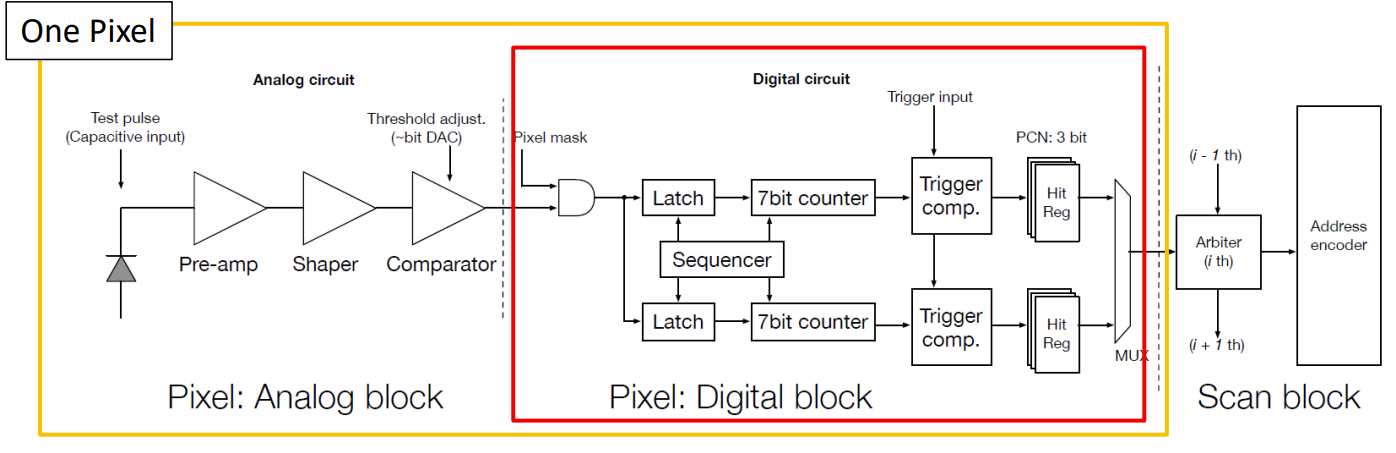
\includegraphics[scale=0.3]{SOI1}}\quad
\subfigure[Operational sketch.]{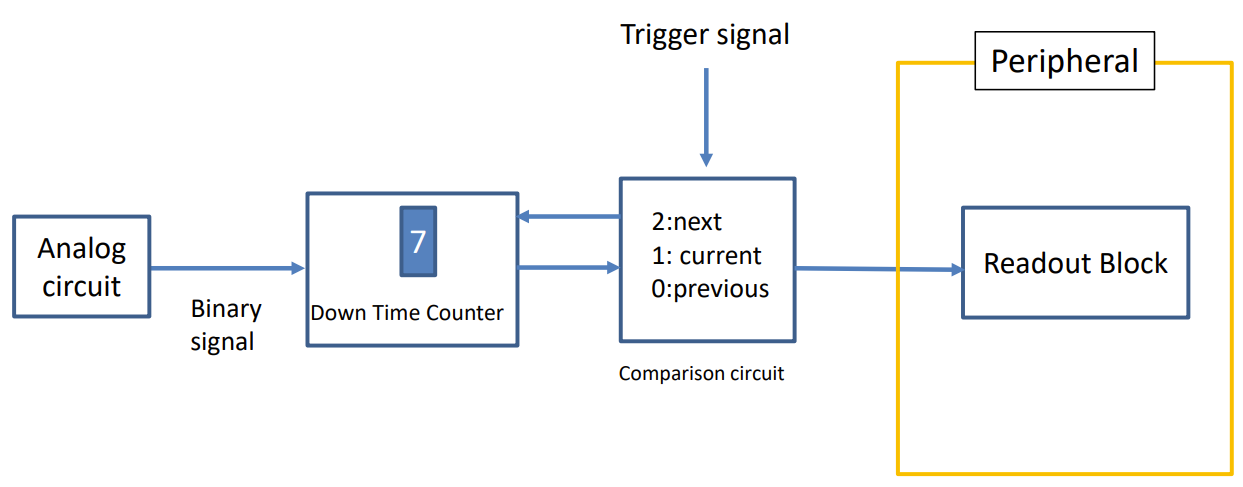
\includegraphics[scale=0.4]{SOI2}}\\
\caption{Schematic of DuTiP circuits.}
\label{SOI}
\end{figure}

\subsubsection{Sensor design and and features}

The size fo the new designed pixel is 45 $\mu$m and the sensor layer thickness of 50 $\mu$m, which gives about 11 $\mu$m of intrinsic resolution on \textit{z} direction averaging over incident polar angle. ALPIDE was choosen as analog circuit with some modification to adapt it to SOI technology. 

DuTiP pixel detector is designed to cover the current VXD acceptance with 7 layer: 1-3 with S (smaller size chip) type sensors, 4-7 with L(larger size) type instead (\vpageref{fig:SL_SOI}).

\begin{figure}[h!]
\centering
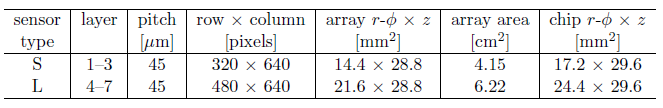
\includegraphics[scale=1]{SL_SOI}
\caption{The size of Small (S) and Large (L) DuTiP chips.}
\label{fig:SL_SOI}
\end{figure}

In order to minimize the dead region between chips in the ladder, stitching technique allows to produce longer chips in the \textit{z} direction, but the structure of the ladders has not be decided yet. For the inner layer of the detector might be possible the cooling with airflow at room temperature; for the outer layers instead, a combination of air and water flows.

For layer 1, which is expected to work in more severe condition of background, the pixel occupancy has been estimated with the trigger latency of 8.0 $\mu$s and both (L and S?) are small enough, O($10^{14}$) or less, thus stabòe tracking and vertexing are contemplated. Moreover without using two timers for layer 1, the signal loss probability with the trigger latency of 4.5 (8.0) $\mu$s is about 0.2 (0.4)\% and so not negligible. In fact if the background rate is higher and the latency is longer, the signal loss probability increases. 

A first prototype of this new desgin has been delivered in June 2021, with all in-pixel functionalitites except for the scan block and the fast readout system. the chip is a matrix of 64x64 pixels and size of 6x6 $mm^{2}$. Its characterization is ongoing and it seems to work fine, aslo with radioactive sources and red laser. A second prototype had been submitted in December 2021, with 64x320 pixels and size of 18x6 $mm^{2}$ (\vpageref{fig:dutip_matrix}). 


\begin{figure}[h!]
\centering
\subfigure[DuTip first prototype.]{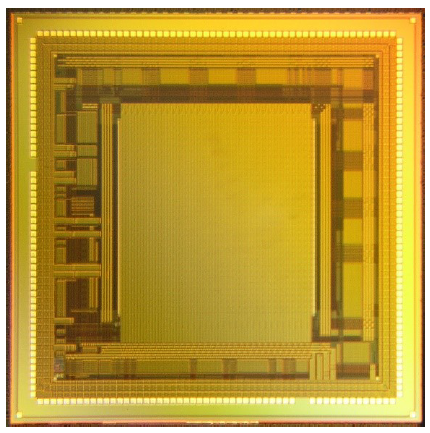
\includegraphics[scale=0.5]{DuTiP1}}\quad
\subfigure[DuTip second prototype.]{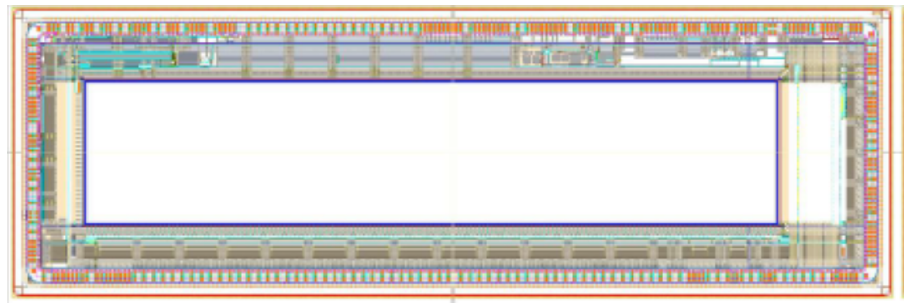
\includegraphics[scale=0.5]{DuTiP2}}\\
\caption{DuTiP prototypes.}
\label{fig:dutip_matrix}
\end{figure}



\subsection{CMOS MAPS}

The last proposal is the one that we will analyze in more details in the next chapters. Like the previous one, it aims to replace the entire current VXD detector using a new technology, in this case the CMOS MAPS, that is Monolithic Active Pixel Sensor CMOS (Complementary Metal-Oxide Semiconductor). \\
The program hopes to solve some of the issues discussed in the previous chapters, with a new system of two inner layers and three outermost, for a total of 5 stages equipped with the same pixel type, called \textbf{VTX} (\vpageref{VTX_layout}). Also the machanical structure had been redesigned but it is expceted that the all system could work at room temperature, so as consequence an important reduction of services is also contemplated.\\
The new pixel design is called OBELIX, based on the pixel matrix of the TJ-Monopix 2 chip, whose characterization is the main topic of this work. 

\begin{figure}[h!]
\centering
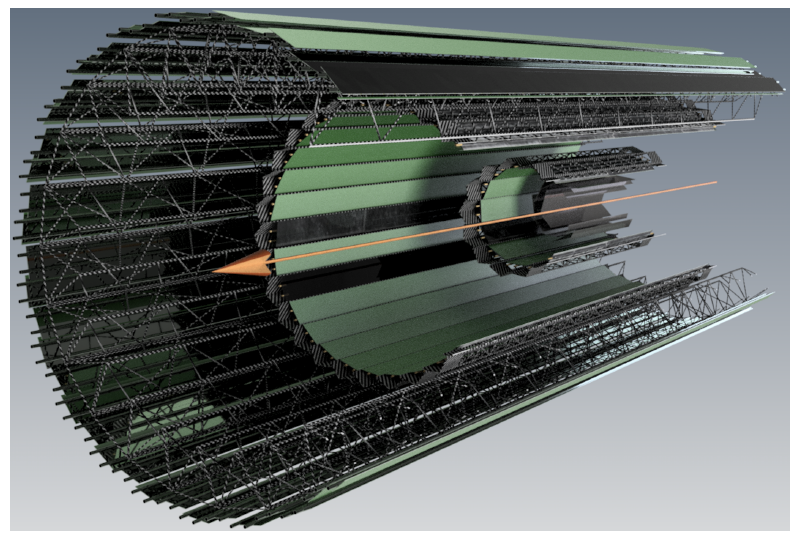
\includegraphics[scale=.6]{VTX_layout}
\caption{Overall VTX layout.}
\label{VTX_layout}
\end{figure}

At the current state of art, intense R\&D(Research and Development) is being carried out, taking advantage from other experiments experiences, like ALICE, with tha same type of sensor.

After a briefly review of the main upgrade proposals, we can now deepen into this last one in the following chapter.



%---------------------------------------------
%			COMMENT
%---------------------------------------------
 %2.1
\begin{comment}
SuperKEKB is already the world's highest-luminosity collider and it aims to reach a new peaks luminosity [of 6.3 $\dot 10^{35}$ $cm^{-2}s^{-1}$] in the future by further increasing the beam-currents and reducing the beam-size at the interaction point by squeezing the betatron function down to $\beta^{*}_{y}$ = 0.3 mm (mentioned in section REFERENCE). For this reason, it's necessary to understand how to mitigate the beam backgrounds where possible and how to cope with the consequent challenges. 
\end{comment}


\begin{comment}
[So it is a of a great importance simulate and measure the background to check on the state of the detector and the machine but also to predict how the conditions could change.]
In figure .... the Belle II background level measured in..... is shown. Current background rates in the experiment are acceptable and above all in most cases well below the limits (listed??). 
\end{comment}
